\section{Diseño y Arquitectura}
GeoDengue está basada en una arquitectura, de tres capas, cliente-servidor, en el que las tareas
se reparten entre los proveedores de recursos o servicios, denominados servidores, y los
demandantes, llamados clientes. La primera capa, la de presentación, es la que se encarga de
interactuar con el usuario final, la segunda capa es la de negocios, esta se encarga de procesar
las solicitudes realizadas por la capa de presentación y definir las reglas que deben aplicase en
para cada solicitud. Por último, se encuentra la capa de datos, donde se almacenan los datos,
procesan las peticiones de la capa de negocios para persistir o recuperar información. En la
\figref{fig:arquitectura-completa} se pude apreciar los componentes del sistema y las interacciones
entre los mismos.

\begin{figure}[!htpb]
\centering
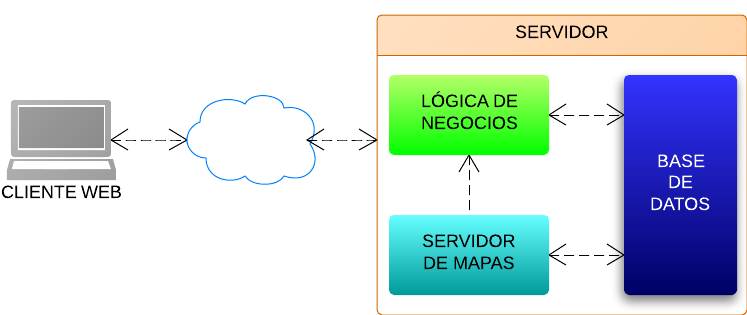
\includegraphics[width=1\textwidth]{capitulo-5/graphics/arquitectura-completa.png}
\caption{\label{fig:arquitectura-completa}Arquitectura de interacción de componentes de GeoDengue.}
\end{figure}

Se optó por un enfoque web debido a la practicidad de estas aplicaciones, el usuario final solo
debe contar con un navegador web. Estas deberían funcionar igual independientemente de la versión
del sistema operativo instalado en el cliente. Las aplicaciones web son catalogadas como
aplicaciones de bajo consumo, debido a que la mayor parte de la aplicación no se encuentra en
el ordenador del cliente, y muchas de las tareas de procesamiento que realiza el software no
consumen recursos del cliente porque se realizan en el servidor.

El Cliente Web se encuentra diseñado como una Aplicación de una Sola Página o SPA (por sus siglas
en ingles Single Page Application), donde la aplicación se ejecuta en una única página, y la
navegación se realiza mediante cargas parciales, sin recargar el sitio completamente.

La capa de negocios se encuentra acompañada por un servidor de mapas que se encarga de publicar y
ofrecer datos geoespaciales. La capa de negocios se comunica con el servidor de mapas para
publicar los resultados de las operaciones realizadas. El Cliente Web, a su vez, se comunica con
la capa de negocios, para realizar operaciones de análisis y procesamiento, y con el servidor de
mapas para obtener los datos geoespaciales publicados.
